% !TEX program = xelatex
\documentclass{article}

\usepackage[final,main]{neurips_2025}

\usepackage{fontspec}
\usepackage{xeCJK}
\setmainfont{TeX Gyre Termes}
\setsansfont{TeX Gyre Heros}
\setmonofont{TeX Gyre Cursor}
\setCJKmainfont{FandolSong-Regular}
\XeTeXlinebreaklocale "zh"
\XeTeXlinebreakskip = 0pt plus 1pt

\usepackage{hyperref}
\usepackage{url}
\usepackage{booktabs}
\usepackage{amsmath}
\usepackage{amsfonts}
\usepackage{amssymb}
\usepackage{microtype}
\usepackage{xcolor}
\usepackage{graphicx}
\usepackage{subcaption}
\usepackage{tabularx}
\usepackage{array}
\usepackage{float}
\usepackage{multirow}
\usepackage{makecell}
\usepackage{caption}
\usepackage{enumitem}

\captionsetup{font=small}
\raggedbottom
\setlist[itemize]{leftmargin=1.5em}
\newcolumntype{L}[1]{>{\raggedright\arraybackslash}p{#1}}
\newcolumntype{C}[1]{>{\centering\arraybackslash}p{#1}}

\newcommand{\githubplaceholder}{\url{https://github.com/chen12138-123/HW3--}}
\newcommand{\weightplaceholder}{\url{https://pan.baidu.com/s/1voGnHTbvz8gjdoWDuJbzug?pwd=mjxn}}
\makeatletter
\renewcommand{\@notice}{}
\makeatother

\title{期末作业题目二：\\基于 LeRobot 的 ACT 策略跨环境泛化挑战}

\author{%
  周湘洋、毛琦骏、陈希
}

\begin{document}

\maketitle

\begin{abstract}
本报告汇报基于 LeRobot 的 ACT 策略在 CALVIN 上的跨环境泛化实验。实验分别训练仅使用环境 A 数据的 \texttt{A-only} 模型与联合使用环境 A+B+C 数据的 \texttt{ABC-joint} 模型，并从训练收敛、未见环境 \texttt{splitD} 上的离线动作误差，以及 \texttt{splitA} 到 \texttt{splitD} 的视觉偏移增量三个层面进行对比。结果显示，\texttt{2000 step} 时两条策略的训练 loss 已进入阶段性稳定区间，而 \texttt{ABC-joint} 在未见环境上的动作误差更低；到 \texttt{10000 step}，\texttt{ABC-joint@10000} 的 \texttt{D-A} gap 从 \texttt{A-only@10000} 的 0.0266 降到 0.0070，重规划一致性增量也从 0.0069 降到 0.0046。上述结果表明，在固定 ACT 架构与动作块长度的条件下，多环境联合训练能够减弱视觉偏移对块首动作和后续动作块一致性的破坏，从而表现出更强的 zero-shot 跨环境鲁棒性。
\end{abstract}

\section{任务背景}

CALVIN 是一个面向长时序机器人操作的开源模拟基准，任务本身依赖视觉输入、连续控制和多步动作衔接 \citep{mees2021calvin}。本实验在 LeRobot 框架中训练 ACT（Action Chunking with Transformers）策略，并比较训练数据的环境覆盖范围对未见环境泛化的影响。

实验比较下面两个模型：
\begin{itemize}
  \item \textbf{\texttt{A-only@10000}}：仅使用环境 A 数据训练，模型在源环境 A 上是否具有更低的动作误差。
  \item \textbf{\texttt{ABC-joint@10000}}：联合使用环境 A+B+C 数据训练，模型在未见环境 D 上是否具有更好的泛化表现。
\end{itemize}

\section{数据集描述}

实验使用已经转换为 LeRobot 格式的 CALVIN 数据。训练时分别使用环境 A，或者把环境 A+B+C 合并；评测时统一放到未见环境 D 上。环境 D 未参与训练。

\begin{table}[H]
  \centering
  \small
  \caption{数据划分与用途。}
  \label{tab:data_splits}
  \begin{tabular}{L{2.0cm}L{3.2cm}C{1.8cm}C{1.8cm}}
    \toprule
    Split & 用途 & 帧数 & Episode 数 \\
    \midrule
    \texttt{splitA} & 训练 \texttt{A-only} & 366,693 & 6,089 \\
    \texttt{splitABC} & 训练 \texttt{ABC-joint} & 1,071,743 & 17,870 \\
    \texttt{splitD} & zero-shot 分析 & 308,918 & 5,124 \\
    \bottomrule
  \end{tabular}
\end{table}

本地数据字段已经整理成 LeRobot v3 的命名风格，主要包括：
\begin{itemize}
  \item 静态相机图像：\texttt{observation.images.image}
  \item 手腕相机图像：\texttt{observation.images.wrist\_image}
  \item 机器人状态：\texttt{observation.state}
  \item 目标动作：\texttt{action}
\end{itemize}

\begin{figure}[H]
  \centering
  \begin{subfigure}[t]{0.62\linewidth}
    \centering
    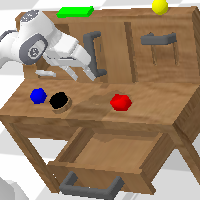
\includegraphics[width=\linewidth]{figures/splitD_sample_static.png}
    \caption{静态相机视角}
  \end{subfigure}
  \hfill
  \begin{subfigure}[t]{0.26\linewidth}
    \centering
    
\includegraphics[width=\linewidth]{figures/splitD_sample_wrist.png}
    \caption{手腕相机视角}
  \end{subfigure}
  \caption{\texttt{splitD} 中一条真实样本的视觉输入示意。对应样本还包含 15 维 \texttt{observation.state} 与 7 维 \texttt{action}。}
  \label{fig:data_example}
\end{figure}

\section{方法原理简述}

实验使用 LeRobot 中集成的 ACT 策略。给定当前时刻的两路相机图像和机器人状态，ACT 不只预测当前一步动作，而是一次输出一段未来动作块（action chunk）。本实验中 chunk size 设为 100，因此每次前向都会生成长度为 100 的连续动作序列。训练阶段使用对应长度的专家动作片段做整段监督；推理阶段执行其中当前时刻对应的动作，并随着新观测到来滚动更新后续动作块。模型主体采用 Transformer，并结合条件变分自编码器（CVAE）式潜变量来吸收同一观测下演示动作的多样性 \citep{zhao2023learning}。

本报告重点观察这一动作块机制在跨环境视觉偏移下的表现。环境 D 与训练环境 A/B/C 保持相同任务语义和动作空间，但场景外观、背景与物体呈现方式发生变化。对单步控制而言，当前图像中的扰动更容易直接传到当前动作；而 ACT 会把当前决策放到一小段连续动作中联合建模，因此更适合用来观察视觉变化出现后，局部动作轨迹是否仍能保持一致。基于这一点，后文主要比较 \texttt{splitA} 与 \texttt{splitD} 上的当前步动作 L1 误差（只比较动作块中的第一个动作）、\texttt{arm/gripper} 分量误差、\texttt{D-A} 泛化落差，以及相邻时刻两次动作块预测在重叠区间上的重规划一致性。

本实验中，策略接收两路视觉输入和一路低维状态输入，输出 7 维连续动作，其中前 6 维对应机械臂，最后 1 维对应夹爪。报告指标包括：
\begin{itemize}
  \item 训练过程 loss 曲线；
  \item \texttt{splitA} 与 \texttt{splitD} 上的离线当前步动作 L1 误差；
  \item \texttt{D-A} 泛化落差；
  \item 相邻时刻动作块重叠区间的重规划一致性；
  \item 分解后的 arm(6D) 与 gripper(1D) 误差。
\end{itemize}

\section{实验设置}

\subsection{训练与硬件设置}

所有实验都在 NVIDIA RTX 4090 48GB GPU 上完成，训练框架为 LeRobot v0.5.1。\texttt{2000 step} 实验用于记录训练与验证曲线，\texttt{10000 step} 模型用于最终性能汇报。两组实验保持相同 ACT 网络结构、batch size、学习率、优化器和随机种子；区别在训练步数与 checkpoint 保存密度。

\begin{table}[H]
  \centering
  \small
  \caption{主要超参数与实验设置。}
  \label{tab:hyperparams}
  \begin{tabular}{L{3.5cm}L{10.0cm}}
    \toprule
    项目 & 配置 \\
    \midrule
    Framework & LeRobot v0.5.1 \\
    Policy & ACT \\
    Visual backbone & \texttt{resnet18}, pretrained weights = \texttt{ResNet18\_Weights.IMAGENET1K\_V1} \\
    Input modalities & 静态相机图像（$3 \times 200 \times 200$）、手腕相机图像（$3 \times 84 \times 84$）、15 维机器人状态 \\
    Output action & 7 维连续动作 \\
    Chunk length / prediction horizon & 100 / 100 \\
    Transformer & \texttt{dim\_model}=512, \texttt{n\_heads}=8, \texttt{dim\_feedforward}=3200 \\
    Encoder / decoder layers & 4 / 1 \\
    Latent modeling & CVAE enabled, latent dim = 32, VAE encoder layers = 4 \\
    Dropout & 0.1 \\
    Loss function & ACT 默认训练目标：动作重建损失 + KL 正则项（\texttt{kl\_weight}=10.0） \\
    Optimizer & AdamW, learning rate = $1\times10^{-5}$, weight decay = $1\times10^{-4}$ \\
    Gradient clipping & 10.0 \\
    Batch size & 32 \\
    Data loading & \texttt{num\_workers}=4, \texttt{video\_backend}=pyav \\
    Random seed & 1000 \\
    Curve runs & \texttt{A-only@2000}, \texttt{ABC-joint@2000}, checkpoints at 500/1000/1500/2000 \\
    Final runs & \texttt{A-only@10000}, \texttt{ABC-joint@10000} \\
    Evaluation set & stratified \texttt{splitA} vs. \texttt{splitD}, 34 shared task families $\times$ 128 samples/family, seed = 0, batch size = 32 \\
    Primary metric & offline current-step action L1 (\texttt{avg\_l1\_loss}, 仅比较动作块第一个动作) \\
    Auxiliary metrics & training loss, \texttt{D-A} gap, replan consistency, arm L1 gap, gripper L1 gap \\
    \bottomrule
  \end{tabular}
\end{table}

\subsection{Checkpoint 与离线评测流程}

\texttt{2000 step} 实验主要用于观察训练前期的变化趋势，因此在 \texttt{500/1000/1500/2000} 四个位置保存 checkpoint。各 checkpoint 保存后，统一运行离线评测。

离线评测先读取 \texttt{splitA} 与 \texttt{splitD} 的任务标签，并按 task family 分组。脚本保留两个 split 中都出现的 34 类任务，在每一类内固定随机种子 \texttt{seed=0}，分别抽取 128 个样本，组成总计 4352 条样本的评测子集。这样比较 \texttt{splitA} 与 \texttt{splitD} 时，任务构成保持一致，视觉偏移带来的误差变化更容易单独观察。

对每个 checkpoint，先在该子集上计算 \texttt{splitD} 的当前步动作 L1 误差；再用同一套采样结果分别计算 \texttt{splitA} 和 \texttt{splitD} 的动作误差，并将两者之差记为 \texttt{D-A} visual shift gap。报告中同时汇报环境 D 的绝对误差和从环境 A 切换到环境 D 后的误差增量。

围绕 ACT 的动作块机制，评测脚本还在每个 family 内额外抽取至多 64 对同一 episode 的相邻帧，比较相邻两帧预测动作块在重叠区间上的 L1 差，并将其记为重规划一致性误差。\texttt{10000 step} 实验不再展开中间 checkpoint 曲线，只使用最终的 \texttt{10000 step} checkpoint 汇报主结果。

\subsection{收敛指标与评价指标}

记专家动作为 $a_t \in \mathbb{R}^7$，ACT 在时刻 $t$ 输出长度为 $H=100$ 的动作块
\[
\hat{A}_t = [\hat{a}_{t,0}, \hat{a}_{t,1}, \ldots, \hat{a}_{t,H-1}],
\]
其中当前时刻实际用于离线评测的预测动作为 $\hat{a}_t=\hat{a}_{t,0}$。

\paragraph{收敛指标：训练 loss}
训练阶段直接使用 LeRobot 日志中的 \texttt{train/loss}。该量对应 ACT 默认训练目标，即动作重建项与 KL 正则项之和：
\[
\mathcal{L}_{\text{train}}=\mathcal{L}_{\text{act}}+\lambda_{\text{KL}}\mathcal{L}_{\text{KL}}.
\]

\paragraph{评价指标：当前步动作 L1 误差}
设评测集共有 $N$ 个样本，则整体动作误差定义为
\[
\mathrm{L1}_{\text{all}}=\frac{1}{7N}\sum_{t=1}^{N}\|\hat{a}_t-a_t\|_1.
\]
前 6 维机械臂误差与第 7 维夹爪误差分别记为
\[
\mathrm{L1}_{\text{arm}}=\frac{1}{6N}\sum_{t=1}^{N}\sum_{d=1}^{6}\left|\hat{a}_t^{(d)}-a_t^{(d)}\right|,
\quad
\mathrm{L1}_{\text{gripper}}=\frac{1}{N}\sum_{t=1}^{N}\left|\hat{a}_t^{(7)}-a_t^{(7)}\right|.
\]

\paragraph{评价指标：Visual shift gap}
对同一模型，分别在 \texttt{splitA} 与 \texttt{splitD} 上计算当前步动作 L1 误差，再定义
\[
\mathrm{Gap}_{D-A}=\mathrm{L1}_{D}-\mathrm{L1}_{A}.
\]
该值越小，说明模型从源环境 A 迁移到未见环境 D 时的误差放大量越小。

\paragraph{评价指标：Replan consistency}
为观察动作块机制本身的稳定性，对同一 episode 中相邻两个时刻 $t$ 与 $t+1$ 的预测动作块，比较其重叠区间
$[\hat{a}_{t,1},\ldots,\hat{a}_{t,H-1}]$ 与 $[\hat{a}_{t+1,0},\ldots,\hat{a}_{t+1,H-2}]$ 的 L1 差。若共有 $M$ 对连续样本，则
\[
\mathrm{RC}_{\text{all}}=
\frac{1}{7(H-1)M}
\sum_{t=1}^{M}
\sum_{k=0}^{H-2}
\left\|\hat{a}_{t,k+1}-\hat{a}_{t+1,k}\right\|_1.
\]
对应地，也分别统计 \texttt{arm} 与 \texttt{gripper} 的重规划一致性误差。该值越小，表示相邻时刻重新规划出的动作块越一致。本文第五章的正式主结果仍以前三类指标为主，Replan consistency 作为补充诊断指标在图 \ref{fig:replan_consistency_10000} 中汇报。

\section{实验结果}

\subsection{训练收敛对比}

训练阶段记录 \texttt{train/loss}；checkpoint 评测阶段记录当前步动作 L1 误差 \texttt{avg\_l1\_loss}。

\begin{table}[H]
  \centering
  \small
  \caption{\texttt{2000 step} 训练收敛对比。}
  \label{tab:train_summary}
  \begin{tabular}{L{2.7cm}C{1.1cm}C{1.3cm}C{1.5cm}C{1.5cm}C{1.3cm}}
    \toprule
    Checkpoint & Points & Epoch frac. & 首3点均值 & 末3点均值 & Final loss \\
    \midrule
    \texttt{A-only@2000} & 10 & 0.17 & 3.1003 & 0.6927 & 0.5950 \\
    \texttt{ABC-joint@2000} & 10 & 0.06 & 3.1167 & 0.6947 & 0.6010 \\
    \bottomrule
  \end{tabular}
\end{table}

\texttt{1500--2000 step} 区间内，两条训练 loss 曲线已经进入缓慢下降阶段，尾段斜率明显小于前半程。这里将“末 3 个记录点均值与 final loss 的相对差小于 15\%”作为阶段性收敛阈值：\texttt{A-only@2000} 的相对差为 $(0.6927-0.5950)/0.6927=14.1\%$，\texttt{ABC-joint@2000} 的相对差为 $(0.6947-0.6010)/0.6947=13.5\%$，两者都落在该阈值以内。因此，本报告将这两组 \texttt{2000 step} 实验记为“已基本收敛”；后续差异更多体现在未见环境上的动作误差，而不是训练目标本身是否继续大幅下降。

\begin{figure}[H]
  \centering
  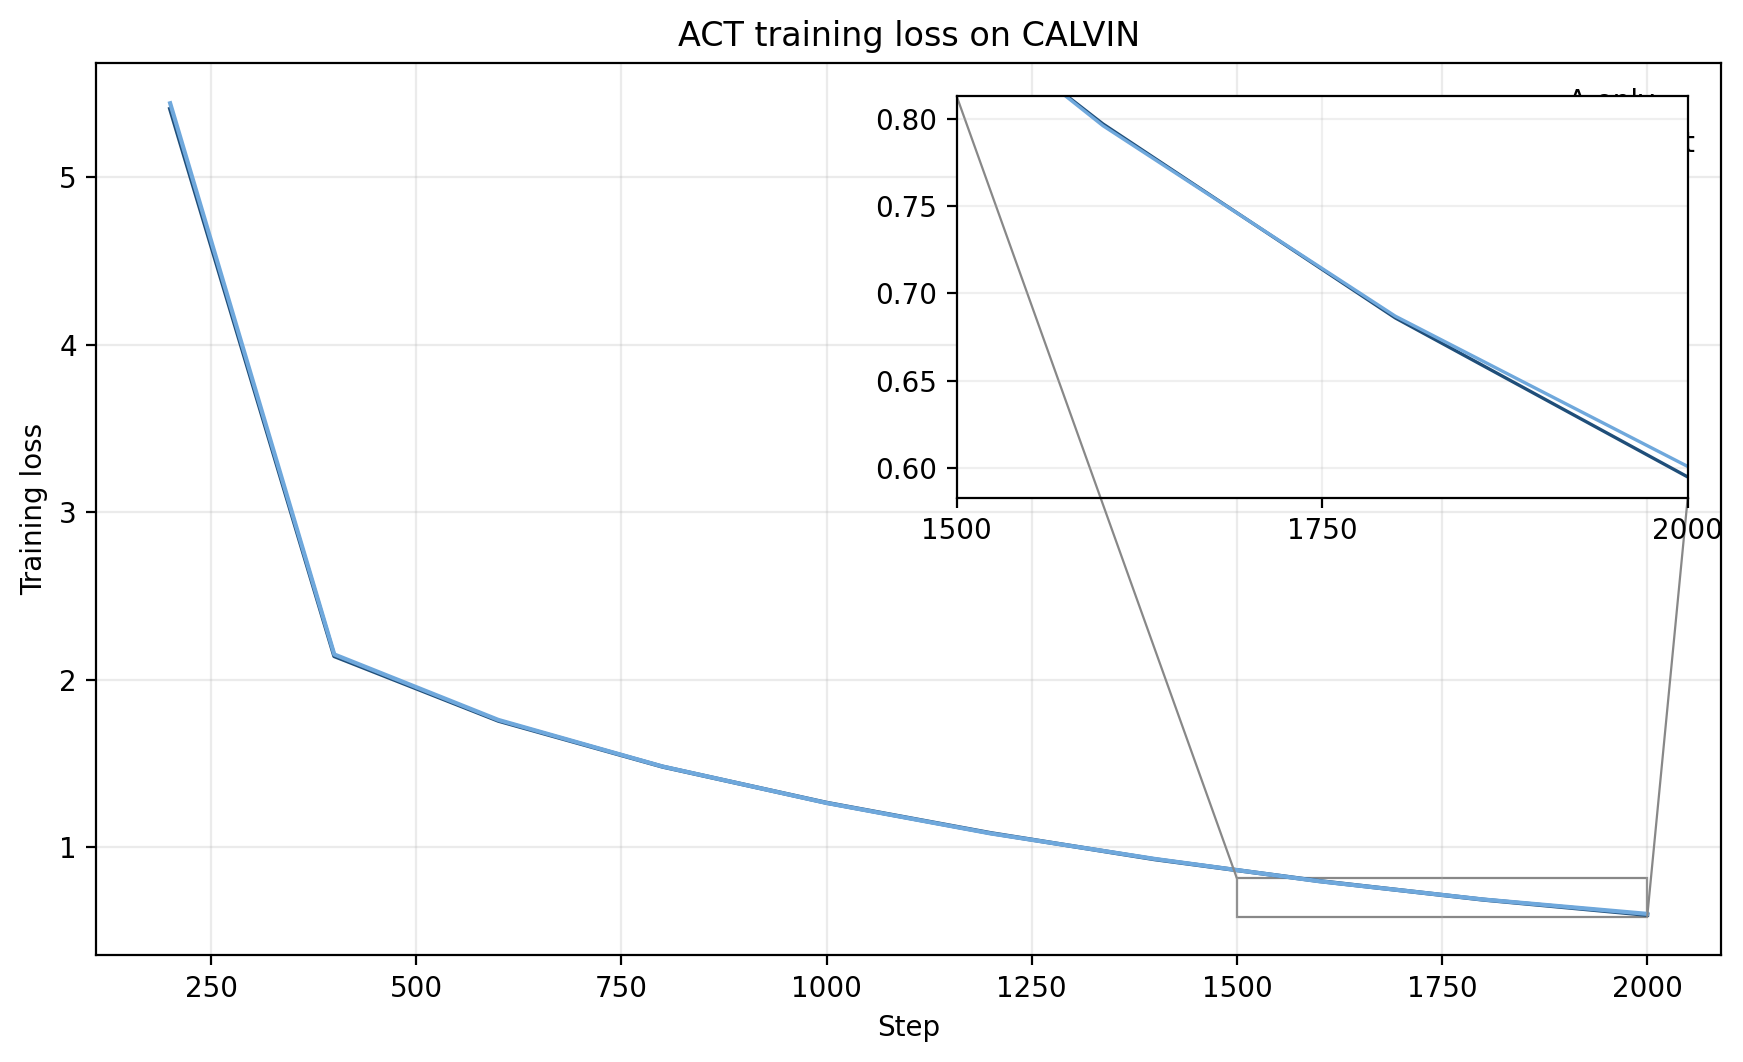
\includegraphics[width=0.94\linewidth]{figures/training_loss_2000_rerun.png}
  \caption{\texttt{2000 step} 训练 loss 对比图，右上角放大 \texttt{1500--2000 step} 尾段。两条曲线整体走势接近，末段差异很小。}
  \label{fig:train_curves}
\end{figure}

\vspace{-1.2em}
\begin{table}[H]
  \centering
  \small
  \caption{\texttt{2000 step} 实验在未见环境 \texttt{splitD} 上的 checkpoint 级动作误差。}
  \label{tab:val_curve_2000}
  \begin{tabular}{L{2.5cm}C{1.0cm}C{1.6cm}C{1.6cm}C{1.6cm}}
    \toprule
    Checkpoint & Step & D avg L1 & D arm L1 & D gripper L1 \\
    \midrule
    \texttt{A-only} & 500 & 0.2653 & 0.1593 & 0.9014 \\
    \texttt{A-only} & 1000 & 0.1686 & 0.1550 & 0.2499 \\
    \texttt{A-only} & 1500 & 0.1611 & 0.1536 & 0.2061 \\
    \texttt{A-only} & 2000 & 0.1536 & 0.1501 & 0.1746 \\
    \texttt{ABC-joint} & 500 & 0.2510 & 0.1596 & 0.7994 \\
    \texttt{ABC-joint} & 1000 & 0.1545 & 0.1544 & 0.1552 \\
    \texttt{ABC-joint} & 1500 & 0.1517 & 0.1539 & 0.1379 \\
    \texttt{ABC-joint} & 2000 & 0.1513 & 0.1505 & 0.1558 \\
    \bottomrule
  \end{tabular}
\end{table}

\subsection{\texttt{2000 step} 验证曲线}

\begin{figure}[H]
  \centering
  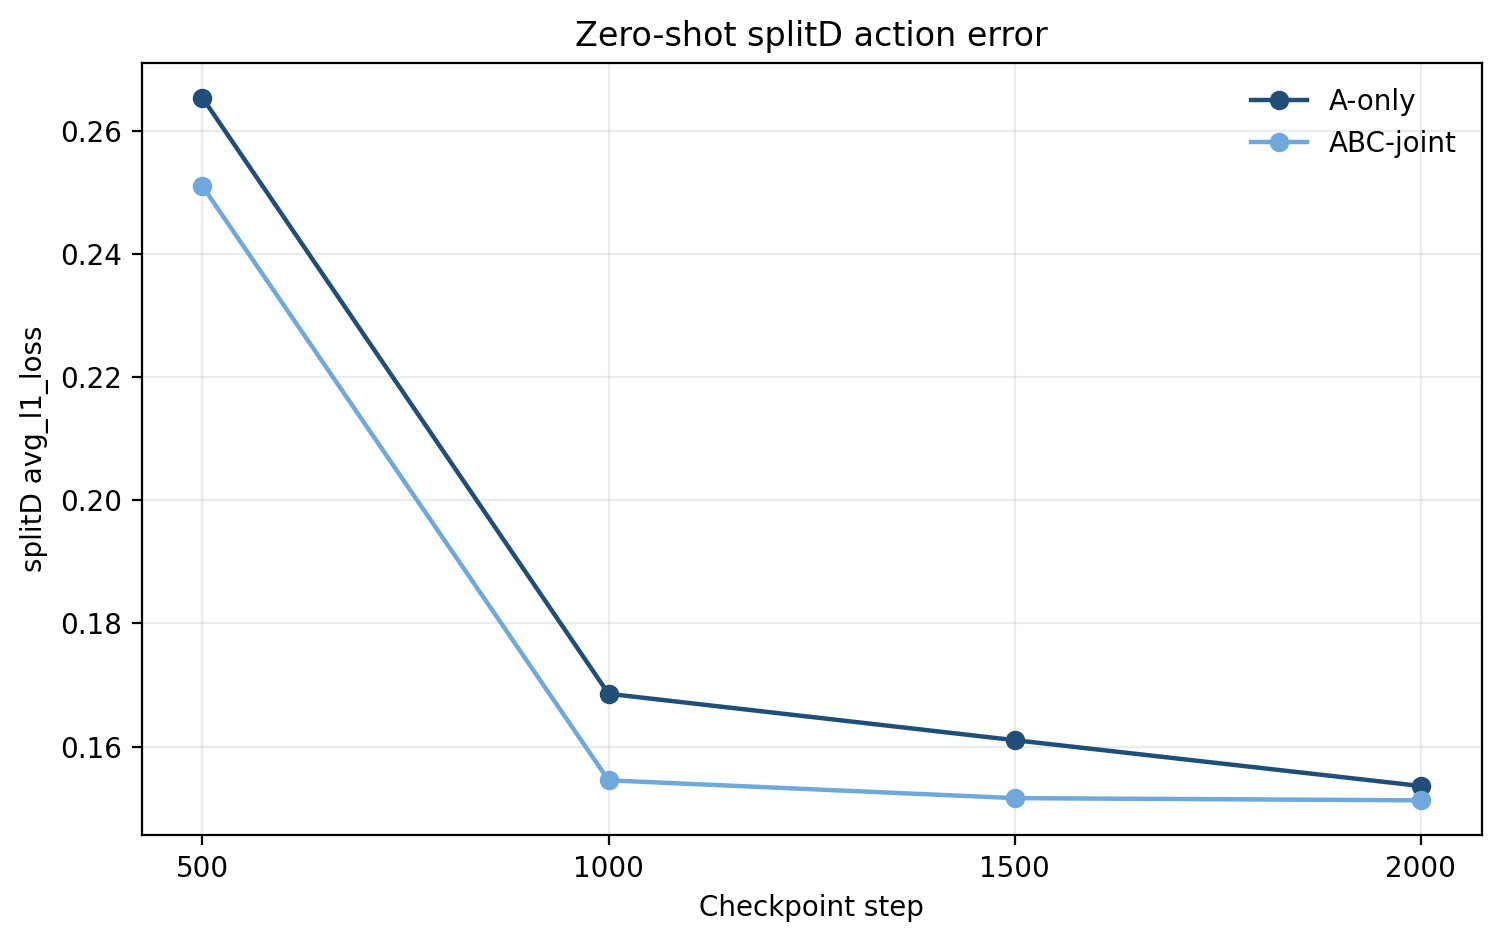
\includegraphics[width=0.74\linewidth]{figures/splitD_avg_l1_2000_rerun.png}
  \caption{\texttt{2000 step} 实验在 \texttt{splitD} 上的 zero-shot 动作误差曲线。两条策略的主要下降发生在 \texttt{500--1000 step}，随后进入较缓慢的改进区间；\texttt{ABC-joint} 在各 checkpoint 上整体略低。}
  \label{fig:splitd_curve_2000}
\end{figure}

\texttt{2000 step} 的 checkpoint 验证结果显示，两条策略在 \texttt{500--1000 step} 区间完成了主要误差下降，之后进入小幅改进阶段。\texttt{ABC-joint} 在 \texttt{splitD} 上的末端动作误差为 0.1513，低于 \texttt{A-only} 的 0.1536；对应的 \texttt{D-A} gap 也从 \texttt{A-only@2000} 的 $+0.0040$ 降到 \texttt{ABC-joint@2000} 的 $-0.0007$。这说明多环境训练带来的跨环境优势在训练中期已经出现，并在后续 checkpoint 中保持稳定。

\subsection{\texttt{10000 step} 最终 zero-shot 泛化结果}

\begin{table}[H]
  \centering
  \small
  \caption{两条 \texttt{10000 step} 最终模型在源环境与未见环境上的关键评价指标。}
  \label{tab:main_results}
  \begin{tabular}{L{2.8cm}C{1.7cm}C{1.7cm}C{1.4cm}C{1.5cm}C{1.5cm}}
    \toprule
    Checkpoint & A avg action L1 & D avg action L1 & D-A gap & D-A arm gap & D-A gripper gap \\
    \midrule
    \texttt{A-only@10000} & 0.1093 & 0.1359 & +0.0266 & +0.0319 & -0.0050 \\
    \texttt{ABC-joint@10000} & 0.1199 & 0.1268 & +0.0070 & +0.0103 & -0.0132 \\
    \bottomrule
  \end{tabular}
\end{table}

表 \ref{tab:main_results} 汇总了最终模型的结果。\texttt{A-only@10000} 在源环境 \texttt{splitA} 上更低，说明单环境训练仍更贴近训练分布；\texttt{ABC-joint@10000} 在未见环境 \texttt{splitD} 上更低，且 \texttt{D-A} gap 从 +0.0266 降到 +0.0070。按绝对值计算，联合训练将跨环境误差增量压缩到单环境训练的约四分之一。

\begin{figure}[H]
  \centering
  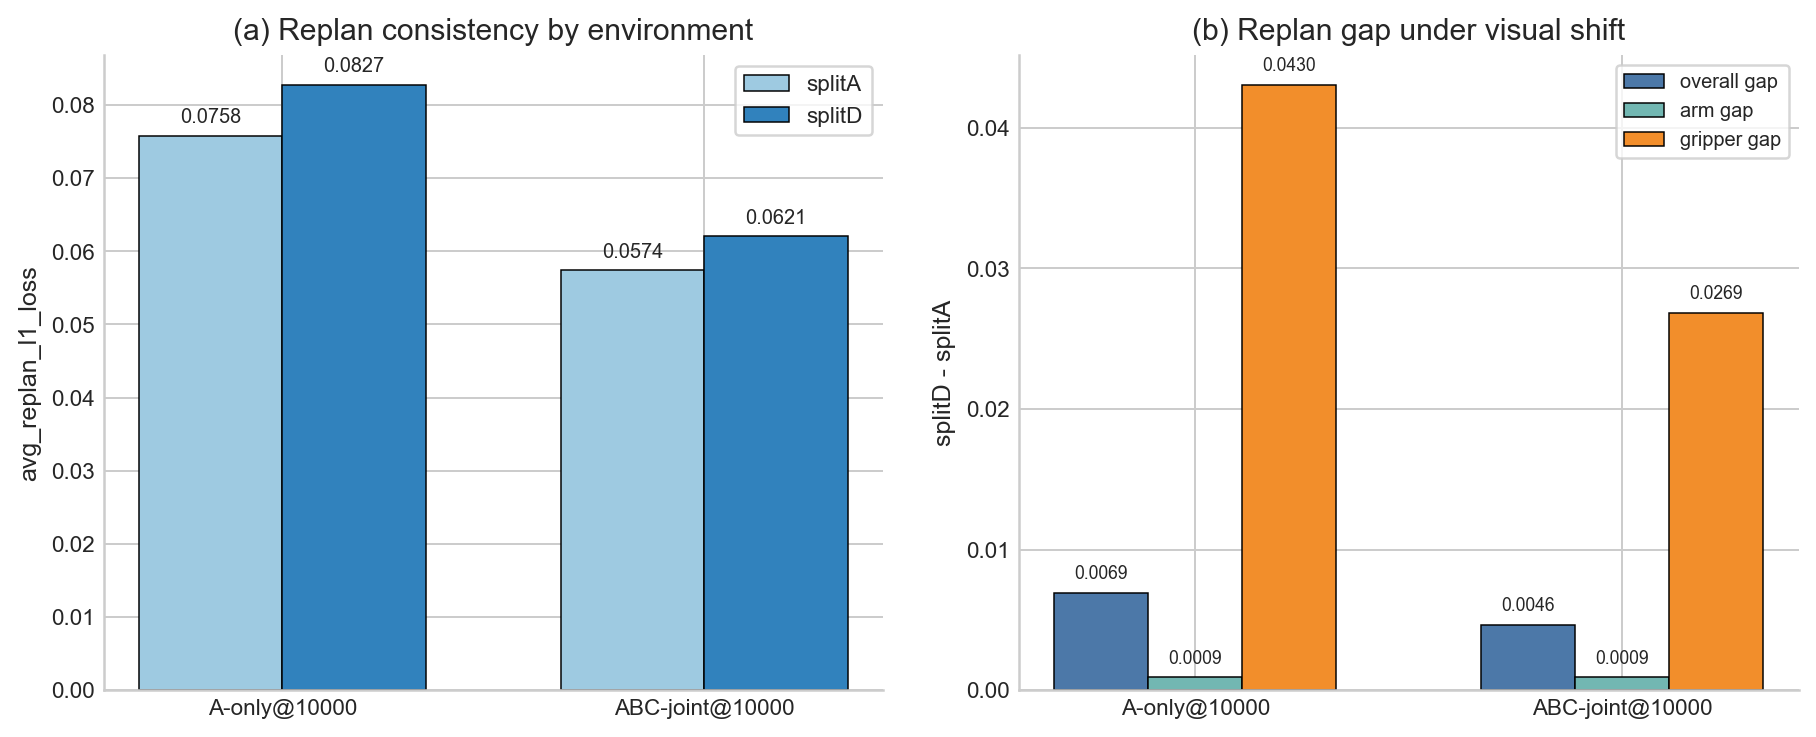
\includegraphics[width=0.98\linewidth]{figures/replan_consistency_10000.png}
  \caption{\texttt{10000 step} 最终模型的重规划一致性结果。左图比较 \texttt{splitA} 与 \texttt{splitD} 上的 \texttt{avg\_replan\_l1\_loss}；右图给出视觉偏移导致的 \texttt{D-A} replan gap 分解。}
  \label{fig:replan_consistency_10000}
\end{figure}

\vspace{-0.5em}
图 \ref{fig:replan_consistency_10000} 直接给出了 Action Chunking 相关的补充证据。\texttt{ABC-joint@10000} 在\texttt{splitA}和\texttt{splitD}上的重规划一致性误差分别为 0.0574 和 0.0621，均低于\texttt{A-only@10000}的 0.0758 和 0.0827；对应的\texttt{D-A} replan gap 也从 0.0069 降到 0.0046。若进一步分解维度，机械臂部分的 replan gap 两者都约为 0.0009，而主要差异来自夹爪维度：\texttt{A-only@10000}的\texttt{gripper} replan gap 为 0.0430，\texttt{ABC-joint@10000}降到 0.0269。

\section{现象分析}

\noindent\textbf{(1) 训练 loss 接近，验证动作误差开始分化。}
\par
\texttt{2000 step} 实验中，两条训练 loss 曲线几乎重合；在\texttt{500--1000 step}区间，\texttt{splitD}动作误差快速下降。随后两条曲线进入缓慢变化阶段：\texttt{ABC-joint}的\texttt{splitD} avg L1 从 0.1545 降到 0.1513，\texttt{A-only}从 0.1686 降到 0.1536。训练优化过程接近，验证误差已经出现稳定差距。

\noindent\textbf{(2) 单环境训练贴近源域，多环境训练适应未见环境。}
\par
\texttt{A-only@10000}在\texttt{splitA}上的动作误差更低，\texttt{ABC-joint@10000}在\texttt{splitD}上的动作误差更低。两者的优势位置不同：单环境训练更贴近源域，多环境训练更适合跨环境部署。

\noindent\textbf{(3) 多环境训练减弱了 A$\rightarrow$D 的退化。}
\par
\texttt{2000 step}曲线中，\texttt{ABC-joint@2000}的\texttt{D-A} gap 为 -0.0007，低于\texttt{A-only@2000}的 +0.0040；\texttt{10000 step}最终模型中，\texttt{ABC-joint@10000}的 gap 为 +0.0070，也低于\texttt{A-only@10000}的 +0.0266。两个训练长度给出一致现象：联合训练降低了从 A 到 D 的跨环境退化。

\noindent\textbf{(4) 动作误差主要体现在 gripper 维度。}
\par
\texttt{500 step}时，两种策略的 gripper L1 都明显高于 arm L1，早期模型对末端夹爪开合的离散状态更不稳定。训练推进到\texttt{1000 step}后，\texttt{ABC-joint}的 gripper L1 从 0.7994 降到 0.1552，下降幅度大于\texttt{A-only}的 0.9014 到 0.2499。这里的 gripper 改善更快，也对应了\texttt{ABC-joint}在\texttt{splitD}总体动作误差上的早期优势。

\noindent\textbf{(5) Action Chunking 的鲁棒性还体现在重规划一致性上。}
\par
ACT 每个时刻都会重新预测长度为 100 的动作块，因此除了块首动作误差之外，还可以比较相邻时刻预测块在重叠区间上的一致性。对本次视觉偏移实验，\texttt{A-only@10000}从\texttt{splitA}到\texttt{splitD}的块首动作误差增加了 0.0266，而\texttt{ABC-joint@10000}只增加了 0.0070；相应的重规划一致性误差增量也从 0.0069 降到 0.0046。两种指标给出同向结论：多环境训练不只减弱了视觉变化传导到当前执行动作的幅度，也减弱了视觉变化对后续动作块内部一致性的破坏。进一步看维度分解，replan gap 的主要来源是\texttt{gripper}，而\texttt{ABC-joint}在这一项上从 0.0430 降到 0.0269，说明动作块在夹爪开合相关决策上更稳。

\section{局限性}

\begin{itemize}
  \item 本报告采用作业允许的 \textbf{action error}，未报告 CALVIN online rollout success rate。
  \item 当前步动作 L1 与相邻重规划一致性都已纳入结果分析；不过重规划一致性目前只做了最终 checkpoint 对比，尚未展开为 checkpoint 曲线或 family 级表格。
  \item 所有模型均使用 ACT，未加入不同 chunk size 或 non-ACT 对照，因此本报告对动作分块机制的分析仍以固定配置下的现象对比为主。
\end{itemize}

\section{外部链接与提交说明}

项目仓库链接和模型权重下载地址如下：

\begin{tabularx}{\linewidth}{@{}L{3.2cm}X@{}}
项目仓库链接 & \href{https://github.com/QijunM0928/lerobot-act-calvin-task2}{\nolinkurl{https://github.com/QijunM0928/lerobot-act-calvin-task2}} \\
模型权重下载地址 & \href{https://pan.baidu.com/s/1voGnHTbvz8gjdoWDuJbzug?pwd=mjxn}{\nolinkurl{https://pan.baidu.com/s/1voGnHTbvz8gjdoWDuJbzug?pwd=mjxn}} \\
\end{tabularx}

本次提交对应的主要权重包括：
\begin{itemize}
  \item \texttt{A-only@2000}
  \item \texttt{ABC-joint@2000}
  \item \texttt{A-only@10000}
  \item \texttt{ABC-joint@10000}
\end{itemize}

\bibliographystyle{plainnat}
\bibliography{refs}

\end{document}
